Se presenta una metodología básica para cualquier proyecto que involucre \hyperlink{abbr}{ML},
esta metodología no es considerada como final o única, sino que funge como
andamiaje para proceder con la aplicación de estas tecnologías. La razón por la
cual se propone una metodología muy general de primera instancia es debido a la
velocidad con la que se desarrolla el campo; como se ha expuesto anteriormente,
antes la fase de Ingeniería de Características era crucial en el proceso, hoy
con el Deep Learning podemos obviar esta fase, esta metodología es modular y no
monolítica; sus pasos se pueden repetir e iterar muchas veces para ajustarla a
resolver el problema (\autoref{fig:metodologia}).

La mayoría de las aplicaciones de \hyperlink{abbr}{ML} se basan en la ingesta de
datos tabulares, es decir, aquellos que se representan cómodamente en un archivo
de Excel. En la actualidad, bastantes más tipos de datos pueden ser utilizados
gracias al \hyperlink{abbr}{DL}. En esta tesis se manejan datos de imágenes pero
también se puede aprender de datos como el audio que cuenta con valores
temporales y su representación es continua.

Esta metodología, con sus siete etapas, es una función que convierte una
problemática en una sistema, el \hyperlink{abbr}{SDAC}. Cada etapa transforma
esta problemática en otra entidad, culminando con un sistema de software que use
el modelo para clasificar células de \hyperlink{abbr}{PAP}, dentro de un
\hyperlink{abbr}{SE}\cite{AurelienGeron2017}:

\begin{enumerate}
    \item El análisis general delimita la problemática, hace una búsqueda de posibles soluciones
    y genera una propuesta de solución.
    \item La obtención de datos se remite a recabar todo lo necesario para convertir la
    propuesta en los datos necesarios para solucionar el problema.
    \item Los datos se necesitan convertir en información, los datos en realidad no son más
    que números en matrices, la información son hechos y proveen contexto.
    \item Pre-procesar la información extrae conocimiento, este genera entendimiento y puede
    ser aprendido.
    \item Al hacer un análisis de algoritmos, podemos convertir el conocimiento
    en algo capaz de ser comprobado mediante un experimento o más, para saber
    que tan efectiva será la solución.
    \item Ajustar el modelo se refiere no solo a entrenarlo, sino de los
    pasos requeridos para asegurar que ese modelo sea el mejor candidato posible
    para la solución.
    \item La implementación convierte un modelo, que no es más que un archivo de computadora,
    en un sistema completo capaz de interactuar con el experto.
\end{enumerate}

\begin{figure}[H]
    \centering
    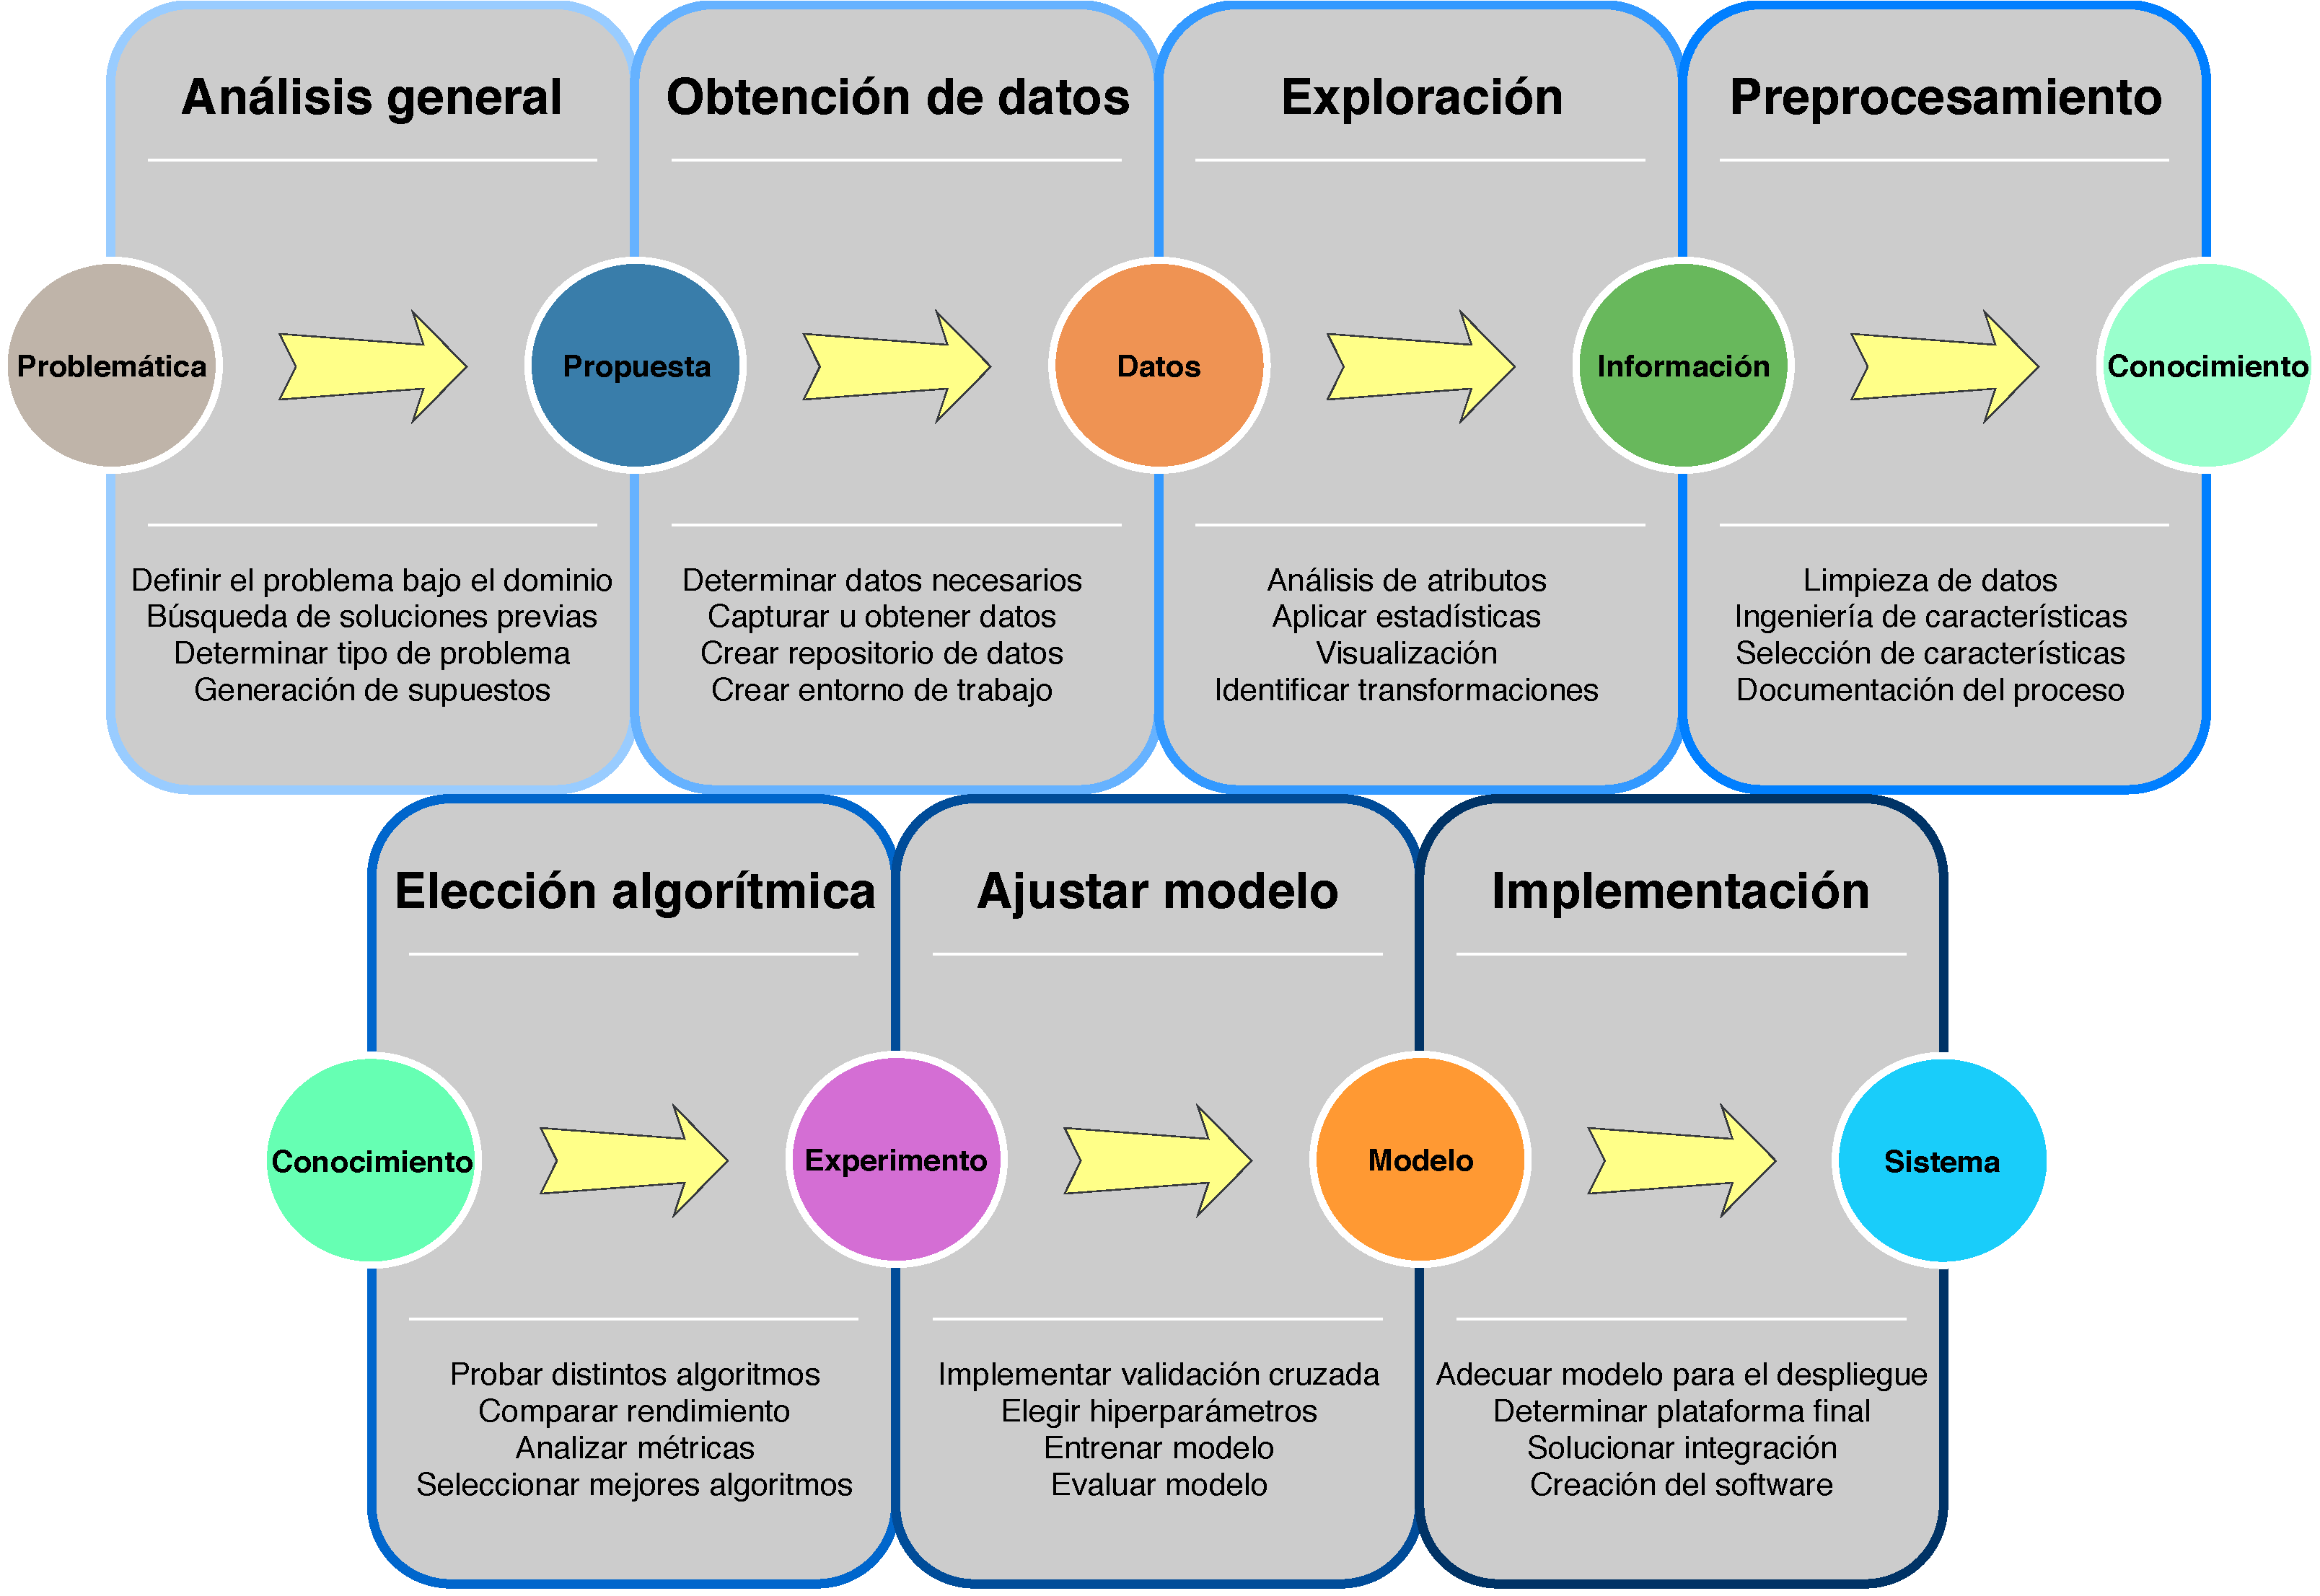
\includegraphics[width=\textwidth]{capitulo_sdac/metodologia_basica_final}
    \caption{Diagrama de la metodología}\label{fig:metodologia}
\end{figure}